\documentclass{article}
\usepackage[utf8]{vietnam}
\usepackage{amsthm}
\usepackage{amsmath}
\usepackage{amsfonts}
\usepackage{amssymb}
\usepackage{graphicx}
\usepackage{url}
\usepackage{cases}

\title{\textbf{Phân tích thiết kế hệ thống "Đăng ký môn học"}}
\author{
  Ngô Quang Dương
}
\date{\today}

\begin{document}

\maketitle

\begin{abstract}
\end{abstract}

\tableofcontents

\section{Mở đầu}

  \subsection{Đặt vấn đề}

  \subsection{Hệ thống hiện tại}

  \subsection{Hướng giải quyết}

\section{Thu thập và phân tích yêu cầu}
  
  \subsection{Bảng thuật ngữ}
    \begin{itemize}
      \item \textbf{Người dùng}: Những người có tài khoản trong hệ thống đăng ký môn học.
      \item \textbf{Sinh viên}: Những người theo học tại trường. Sinh viên theo học một khoa nào đó.
      \item \textbf{Chuyên viên}: Những người làm việc ở phòng công tác sinh viên.
      \item \textbf{Giảng viên}: Người tham gia vào việc giảng dạy. Giảng viên thuộc một khoa nào đó hoặc không. Trong một học kỳ, giảng viên có thể giảng dạy một số môn học tại một số lớp. Tuy nhiên giảng viên chỉ dạy môn học thuộc khoa của mình.
      \item \textbf{Khoa}: Đơn vị mà giảng viên làm việc, sinh viên theo học.
      \item \textbf{Môn học}: Phần kiến thức chuyên về một mảng nào đó, ví dụ như \textbf{giải tích}, \textbf{toán rời rạc}, \textbf{lập trình hướng đối tượng}, \ldots Một môn học có thể thuộc một khoa nào đó hoặc không.
      \item \textbf{Lớp môn học}: Một môn học có thể được chia ra làm nhiều lớp. Chẳng hạn với môn cơ sở dữ liệu (mã môn học là \textbf{INT2207}) có các lớp \textbf{INT2207 1}, \textbf{INT2207 2}, \textbf{INT2207 3}, \ldots
      \item \textbf{Buổi lý thuyết}: Mọi lớp học đều có duy nhất một buổi lý thuyết.
      \item \textbf{Buổi thực hành}: Một lớp học có thể có nhiều hoặc không có buổi thực hành nào.
    \end{itemize}
  
  \subsection{Tác nhân hệ thống}
    \begin{itemize}
      \item Quản trị hệ thống.
      \item Sinh viên.
      \item Chuyên viên.
      \item Giảng viên.
    \end{itemize}
  
  \subsection{Yêu cầu chức năng}
    \paragraph{Chức năng chung:}
    \begin{itemize}
      \item Đăng nhập/đăng xuất.
      \item Chỉnh sửa thông tin tài khoản.
    \end{itemize}

    \paragraph{Chức năng dành cho quản trị hệ thống:}
    \begin{itemize}
      \item Quản lý người dùng.
      \begin{itemize}
        \item Xem thông tin người dùng.
        \item Tìm kiếm người dùng.
        \item Tạo người dùng mới.
        \item Chỉnh sửa thông tin.
        \item Xóa người dùng.
      \end{itemize}
      \item Quản lý môn học:
      \begin{itemize}
        \item Xem thông tin môn học.
        \item Tìm kiếm môn học.
        \item Tạo môn học/lớp môn học mới.
        \item Chỉnh sửa thông tin môn học/lớp môn học.
        \item Xóa môn học/lớp môn học.
      \end{itemize}
      \item Quản lý lớp học:
      \begin{itemize}
        \item Xem thông tin lớp học.
        \item Tìm kiếm lớp học.
        \item Tạo lớp học mới.
        \item Chỉnh sửa thông tin lớp học.
        \item Xóa lớp học.
      \end{itemize}
      \item Mở/đóng hệ thống:
      \begin{itemize}
        \item Cho sinh viên đăng ký môn học.
        \item Cho giảng viên sắp xếp thời khóa biểu.
      \end{itemize}
    \end{itemize}

    \paragraph{Chức năng dành cho sinh viên:}
    \begin{itemize}
      \item Xem thông tin môn học.
      \item Tìm kiếm môn học.
      \item Đăng ký môn học.
      \item Xem thông tin giảng viên.
      \item Tìm kiếm giảng viên.
      \begin{itemize}
        \item Đăng ký môn học mới.
        \item Bỏ môn học đã chọn.
        \item Xem danh sách các môn đã đăng ký.
      \end{itemize}
    \end{itemize}

    \paragraph{Chức năng dành cho chuyên viên:}
    \begin{itemize}
      \item Tìm kiếm sinh viên.
      \item Xem thông tin sinh viên.
      \item Tất cả các chức năng dành cho sinh viên (tuy nhiên việc đăng ký môn học được coi là đăng ký cho sinh viên chứ không phải cho chuyên viên).
    \end{itemize}

    \paragraph{Chức năng dành cho giảng viên:}
    \begin{itemize}
      \item Xem thông tin lớp học.
      \item Tìm kiếm lớp học.
      \item Chọn/hủy lớp giảng dạy.
      \item Đặt thời khóa biểu.
      \item Xem danh sách các lớp đã nhận.
    \end{itemize}

  \subsection{Yêu cầu phi chức năng}
    \paragraph{
      \textnormal{
        Qua khảo sát đối với người dùng là sinh viên, hệ thống cần được đáp ứng các yêu cầu sau:
      }
    }
    \begin{itemize}
      \item Kết nối nhanh.
      \item Thời gian thực.
      \item Giao diện dễ sử dụng.
      \item Dễ tìm kiếm môn học cần đăng ký.
    \end{itemize}
  
  \subsection{Điều kiện ràng buộc}
    \paragraph{Đối với sinh viên và chuyên viên:}
    \begin{itemize}
      \item Không đăng ký quá 2 môn giáo dục thể chất.
      \item Không đăng ký môn học đã qua với điểm cao hơn $ D $.
      \item Không đăng ký 2 môn học trùng thời khóa biểu.
      \item Số tín chỉ không vượt quá $ 40 $.
    \end{itemize}

    \paragraph{Đối với giảng viên:}
    \begin{itemize}
      \item Không nhận hai lớp bị trùng thời khóa biểu.
    \end{itemize}

\section{Đặc tả yêu cầu}

  \subsection{Sơ đồ use case}

  \begin{figure}[!ht]
    \centering
    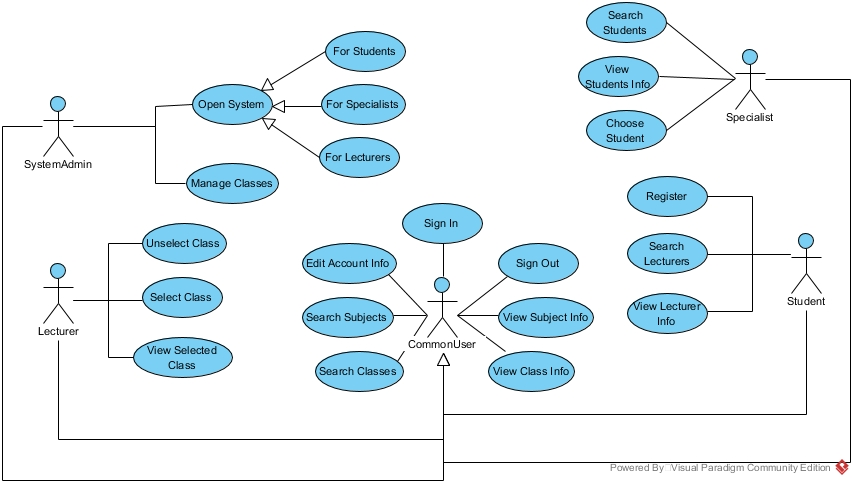
\includegraphics[scale=0.4]{../pictures/projectdiagrams/uc.jpg}
    \caption{Sơ đồ use case}
  \end{figure}

  \begin{figure}[!ht]
    \centering
    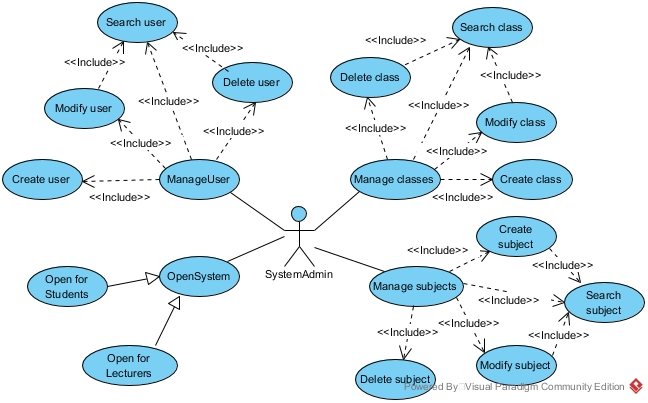
\includegraphics[scale=0.4]{../pictures/projectdiagrams/uc-destructing.jpg}
    \caption{Sơ đồ use case phân rã}
  \end{figure}

  \subsection{Đặc tả use case dưới dạng bảng}

  \paragraph{Các use case chung:}

  \paragraph{Dành cho quản trị hệ thống:}

  \paragraph{Dành cho sinh viên:}

  \paragraph{Dành cho chuyên viên:}

  \paragraph{Dành cho giảng viên:}

  \subsection{Sơ đồ hoạt động}

\section{Phân tích tĩnh}

  \subsection{Xác định lớp}

  \subsection{Quan hệ giữa các lớp}

  \subsection{Lớp phân tích}

  \subsection{Xác định thuộc tính}

  \subsection{Xác định phương thức}

  % \begin{figure}[!ht]
  %   \centering
  %   \includegraphics[]{}
  %   \caption{Sơ đồ lớp}
  % \end{center}

\section{Phân tích động}

  \subsection{Sơ đồ tuần tự}

\end{document}
